% --------------------------------------------------------------- %
%%                                                               %%
%%%                                                             %%%
%%                                                               %%
% --------------------------------------------------------------- %
%
\section{Description of deliverable}

After implementation and internal release of the prototype implementation of the
software framework, the software has undergone testing before making a first
public release.

Testing has been carried out on simple, generic examples and a baseline
application for an expanding polyurethane foam which has been augmented with
multi-scale capabilites using the MoDeNa software framework. The model includes
a simple but realistic representation of the polymerization kinetics and
accounts for the presence of a physical and chemical blowing agent.

The work has been carried out within task 5.5.


% --------------------------------------------------------------- %
%%                                                               %%
%%%                                                             %%%
%%                                                               %%
% --------------------------------------------------------------- %
\section{Summary of contribution of involved partners}
%
WIKKI carried out the implementation of the software framework and two tank
example. NTNU contributed a documentation of the database structure and two tank
example.  POLITO contributed the 0D model and testing resuls. The deliverable
forms the basis of the first release and will be used by used by POLITO, BASF,
VCSHT, US and UNITS for the implementation of the recipies and adaptors for the
demonstration cases.

% --------------------------------------------------------------- %
%%                                                               %%
%%%                                                             %%%
%%                                                               %%
% --------------------------------------------------------------- %
\section{Introduction}
%
The {\MoDeNa} project aims at developing, demonstrating and assessing an
easy-to-use multi-scale software framework application under an open-source
licensing scheme that delivers models with feasible computational loads for
process and product design of complex materials. The concept of {\MoDeNa} is an
interconnected multi-scale software framework. Four scales will be linked
together by this framework namely the nano-, micro-, meso-, and macroscale (see
Figure \ref{fig:ConceptualStructure}).  As application cases we consider
polyurethane foams (PU), which are excellent examples of a large turnover
product produced in a variety of qualities and of which the properties are the
result of designing and controlling the material structure on all levels of
scale, from the molecule to the final product.

\begin{figure}
\centering
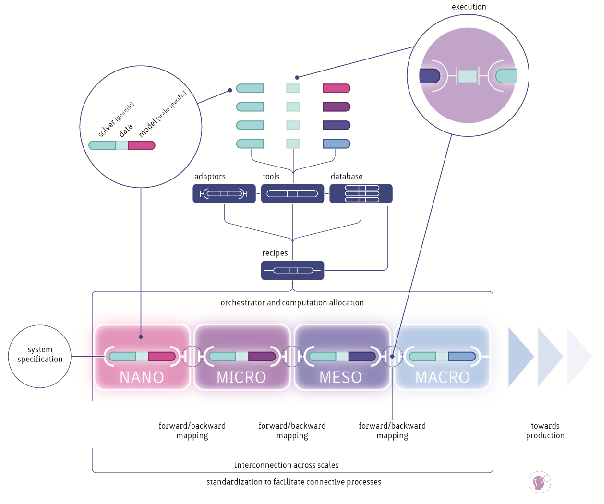
\includegraphics[width=0.70\textwidth]{./Content/Figures/conceptual_structure.eps}
\caption{Conceptual structure of {\MoDeNa}, coupling applications and surrogate
  models into tools, which form sequences through recipes and the orchestrator.}
\label{fig:ConceptualStructure}
\end{figure}

Multi-scale coupling requires the exchange of information between software
instances developed for specific scales in a consistent way. In order to achieve
this, generating consistent representations for models and data is necessary.
The information exchange is governed by protocols and may occur in two ways,
namely:
\begin{itemize}
\item "forward mapping" (passing information from the microscopic to the
  macroscopic scale in upward direction)
\item "backward mapping" (passing information from the macroscopic to the
  microscopic scale in downward direction)
\end{itemize}
``Forward mapping'' is relatively straightforward, while ``backward mapping''
inevitably requires iteration since changing the operating conditions at the
fine level changes the feedback to the coarse level.  ``Backward mapping'' can
be realised by ``two-way coupling'' or by ``fitting surrogate models''. The
first approach usually requires exchange of large amounts of data during runtime
that may be expensive either due to the complexity of the data exchange or the
computational cost associated with executing the microscopic-scale simulation.
In such cases, replacing the microscopic-scale simulation with a surrogate model
presents the only viable alternative. This operation inherently constitutes a
transfer of data across scales and {\MoDeNa} is unique in that it focuses on
this approach.

A typical operation sequence starts a macroscopic-scale simulation which
instantiates one or more surrogate models. When the validity of a model is
violated, a design of experiment operation is triggered. It creates inputs for a
set of microscopic-scale simulations.  When all experiments are finished, the
parameter estimation component is invoked which updates the model parameters.
Next, the macroscopic-scale simulation is restarted. It should be noted, that
the {\MoDeNa} software framework supports application and model dependencies
across multiple scales.
